\subsection{Discounted Dividend Valuations}

\begin{definition} \hlt{Dividends as Definition of Cash Flow}
\begin{enumerate}[label=\roman*.]
\setlength{\itemsep}{0pt}
\item Advantages: theoretically justified, as shareholder's investment today is worth the present value of future cash flows he expects to receive, which is repaid in form of dividends. Dividends are also less volatile than other measures, value estimates based on DDMs are less volatile and reflect long-term earning potential.
\item Disadvantages: not all firms pay dividends. Even by forecasting to the point when the firm is expected to begin paying dividends, there is uncertainty with forecasting that far into the future. Also, minority investors cannot control dividend policy. If dividend policy is not related to firm's ability to create value, then dividends are not an appropriate measure of expected cash flow to shareholders.
\end{enumerate}
Dividends are appropriate as measure of cash flow:
\begin{enumerate}[label=\roman*.]
\setlength{\itemsep}{0pt}
\item Company has history of dividends
\item Dividend policy is clear and related to earnings of the firm
\item Perspective is that of a minority shareholder
\end{enumerate}
Firms in mature stage are likely to meet first two criterial
\end{definition}

\begin{definition} \hlt{Free Cash Flow as Definition of Cash Flow}\\
FCFF is cash flow generated by operations in excess of capital investment required to sustain firm's current productive capacity. FCFE is cash available to shareholders after funding capital requirements and expenses associated with debt financing.
\begin{enumerate}[label=\roman*.]
\setlength{\itemsep}{0pt}
\item Advantage: may be applied to firms with different dividend policies or capital structures. Applicable to controlling shareholders as they may influence distribution and application of free cash flow. For minority shareholders, useful if firm is acquired for market price equal to value to controlling party.
\item Disadvantage: firms with significant capital requirements that may have negative FCF, caused by technological revolution in industry that requires greater investment to remain competitive, or by rapid expansion into untapped markets.
\end{enumerate}
FCF models are most appropriate:
\begin{enumerate}[label=\roman*.]
\setlength{\itemsep}{0pt}
\item For firms with no dividend payment history, or if dividend payment history is not related to earnings
\item For firms wth FCF that corresponds with their profitability
\item Perspective is that of a majority shareholder
\end{enumerate}
\end{definition}

\begin{definition} \hlt{Residual income as Definition of Cash Flow}\\
Earnings exceeding investor's required return.
\begin{enumerate}[label=\roman*.]
\setlength{\itemsep}{0pt}
\item Advantage: theoretically justified, as required return is the opportunity cost to suppliers of capital, and residual income is amount generated in excess of this return. Can be applied to firms with negative FCF and to dividend, and non-dividend paying firms.
\item Disadvantage: require in-depth analysis of accounting accruals, where there may be management discretion for both income and expense. If accounting is not transparent or if quality of firm's reporting is poor, accurate estimation of residual income is difficult.
\end{enumerate}
Residual income approach is most appropriate for:
\begin{enumerate}[label=\roman*.]
\setlength{\itemsep}{0pt}
\item firms with no dividend histories
\item firms with negative FCF for the foreseeable future, due to capital demands
\item firms with transparent financial reporting and high-quality earnings
\end{enumerate}
\end{definition}

\begin{definition} \hlt{Multiple Period Dividend Discount Model}
\begin{equation}
V_0 = \sum\limits_{t=1}^n \frac{D_t}{(1+r)^t} + \frac{P_n}{(1+r)^n} \nonumber
\end{equation}
where $V_0$ is value of share today, $P_n$ is expected price per share to time $n$, $D_t$ is expected dividend per share at end of year $t$, $r$ is required rate of return of stock. 
\end{definition}

\begin{definition} \hlt{Gordon Growth Model}\\
Assumes dividends increase at constant rate indefinitely. 
\begin{equation}
V_0 = \frac{D_0 \times (1+g)}{r-g} = \frac{D_1}{r-g} \nonumber
\end{equation}
where $g$ is expected constant growth rate, and $g < r$.\\
Firm's growth rate projection can be compared to growth rate of economy. Unrealistic to assume that any firm can grow indefinitely at rate higher than long-term growth rate in real GDP plus long-term inflation rate.\\
In general, perpetual dividend growth rate above $5\%$ is suspicious.\\
\end{definition}

\begin{remark} \hlt{Share Repurchases on DDM}\\
If companies have share repurchase programs, use total payout (dividends plus repurchases) in valuation model.\\
Alternatively, DDM focusing on cash dividends can be used after adjusting for number of shares outstanding, taking share repurchases into account.
\end{remark}

\begin{remark} \hlt{Value of Non-Callable Fixed-Rate Perpetual Preferred Stock (Capitalisation Rate)}\\
Firm with no additional opportunities to earn returns in excess of required rate of return should distribute all earnings to shareholders in form of dividends. Hence, growth rate will be zero.
\begin{equation}
V_0 = \frac{D}{r} \nonumber
\end{equation}
where $r$ is the discount rate that capitalises the amount $D$ (level dividend).
\end{remark}

\begin{remark} \hlt{Gordon Growth Model Strengths}
\begin{enumerate}[label=\roman*.]
\setlength{\itemsep}{0pt}
\item Applicable to stable, mature, dividend-paying firms
\item Appropriate for valuing market indices
\item Easily communicated and explained due to straightforward approach
\item Can be used to determine price-implied growth rate, required rates of return, value of growth opportunities
\item Can be used to supplement other more complex valuation methods.
\end{enumerate}
\end{remark}

\begin{remark} \hlt{Gordon Growth Model Weaknesses}
\begin{enumerate}[label=\roman*.]
\setlength{\itemsep}{0pt}
\item Valuations are very sensitive to estimates of growth rates and required rates of return
\item Model cannot be easily applied to non-dividend-paying stocks
\item Unpredictable growth patterns of some firms will make model valuations unreliable
\end{enumerate}
\end{remark}

\begin{remark} \hlt{Implied Growth Rates from Gordon Growth Model}\\
Price, current dividend may be observed for publicly traded stock.\\
Assuming a required return, we may calculate the implied growth rate. 
\begin{equation}
r = \frac{D_1}{P_0} + g \nonumber
\end{equation}
\end{remark}

\begin{remark} \hlt{Present Value of Growth Opportunities (PVGO)}\\
Firm with opportunities to earn in excess of required rate of return will retain earnings to invest in growth opportunities. The valuation will then have PVGO as an additional component.
\begin{equation}
V_0 = \frac{E_1}{r} + PVGO \nonumber
\end{equation}
where $E_1/r$ is the no-growth value per share.\\
Growth companies will have substantial portion of value in PVGO, while companies in slow-growth industries will have low PVGO, where most of their value comes from assets in place.
\end{remark}

\begin{remark} \hlt{Price to Earnings Ratio}\\
A justified P/E ratio is fair, warranted, or justified on the basis of fundamentals.
\begin{enumerate}[label=\roman*.]
\setlength{\itemsep}{0pt}
\item Justified Leading P/E: based on earnings forecast for next period.
\begin{equation}
\text{Justified Leading P/E} = \frac{P_0}{E_1} = \frac{D_1/E_1}{r-g} = \frac{1-b}{r-g} \nonumber
\end{equation}
\item Justified Trailing P/E: based on earnings for previous period.
\begin{equation}
\text{Justified Trailing P/E} = \frac{P_0}{E_0} = \frac{D_0(1+g)/E_1}{r-g} = \frac{(1-b)(1+g)}{r-g} \nonumber
\end{equation}
where $E_t$ is earnings at time $t$, $b$ is retention ratio, $(1-b)$ is dividend payout ratio.\\
Note that the price are the fundamental value of stock derived from Gordon Growth Model.\\
If earnings are expected to grow, $E_1 > E_0$, then the justified trailing P/E will be larger than the justified leading P/E due to the smaller denominator.
\end{enumerate}
\end{remark}

\begin{remark} \hlt{Growth Phases for Companies}\\
A justified P/E ratio is fair, warranted, or justified on the basis of fundamentals.
\begin{enumerate}[label=\roman*.]
\setlength{\itemsep}{0pt}
\item Growth Phase: firm has rapidly increasing earnings, little or no dividends, heavy reinvestment
\item Transition Phase: earnings and dividends still increasing but at a slower rate
\item Mature Phase: earnings grow at stable but slower rate, payout ratios are stabilising as reinvestment matches depreciation and asset maintenance requirements
\end{enumerate}
\end{remark}

\begin{flushleft}
\begin{tabularx}{\textwidth}{p{11em}|p{10.5em}|p{12em}|X}
\hline
\rowcolor{gray!30}
Variable & Growth & Transition & Mature \\
\hline 
Earnings Growth & Very High & Above average, decreasing & Stable at long-run level \\
\hline
Capital Investment & Significant requirements & Decreasing & Stable at long-run level \\
\hline
Profit Margin & High &  Above average, decreasing & Stable at long-run level \\
\hline
FCFE & Negative & Maybe position, growing & Stable at long-run level \\
\hline
ROE vs Required Return & $ROE > r$ & $ROE \rightarrow r$ & $ROE = r$ \\
\hline
Dividend Payout & Low or zero & Increasing & Stable at long-run level \\
\hline
Appropriate Model & Three-stage & Two-stage & Gordon Growth \\
\hline
\end{tabularx} 
\end{flushleft}

\begin{method} \hlt{Two-Stage DDM}\\
Company grows at high rate for relatively short period of time, then reverts to long-run perpetual growth rate.\\
Length of high-growth phase is function of visibility of company's operations.
\begin{equation}
V_0 = \sum\limits_{t=1}^n \frac{D_0 (1+g_S)^t}{(1+r)^t} + \frac{D_0 (1+g_S)^n (1+g_L)}{(1+r)^n (r-g_L)} \nonumber
\end{equation}
where $g_S$ is growth rate in stage one $g_L$ is growth rate in stage two.\\
For a firm that doesn't pay dividends, the first stage dividend is set to zero, then computed.
\end{method}

\begin{figure}[H]
\centering
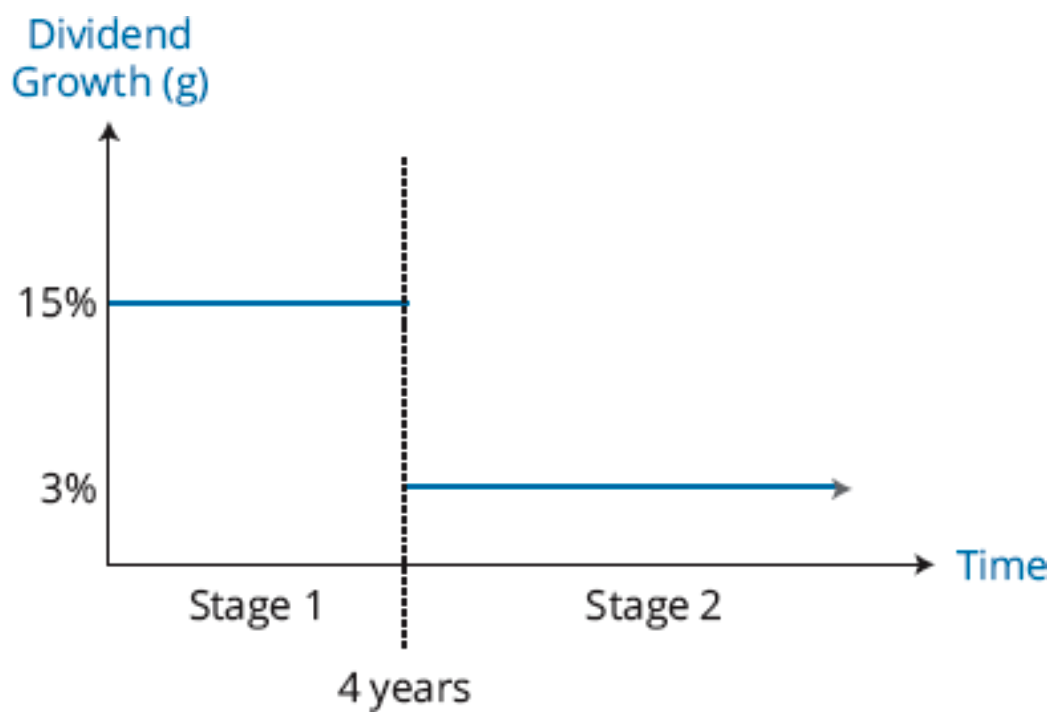
\includegraphics[scale=0.4]{images/equity/twostage}
\caption{Example of a two-stage model}
\end{figure}

\begin{method} \hlt{H-Model DDM}\\
Growth rate starts high, declines linearly over the high-growth stage until the long-run average growth rate.
\begin{equation}
V_0 = \frac{D_0 (1+g_L)}{r-g_L} + \frac{D_0 H (g_S - g_L)}{r-g_L} = \frac{D_0 (1+g_L) + D_0 H (g_S - g_L)}{r - g_L} \nonumber
\end{equation}
where $g_S$ is growth rate in stage one, $g_L$ is growth rate in stage two, $H$ is half-life in years of stage one.\\
The model may be rewritten to solve for $r$:
\begin{equation}
r = \frac{D_0}{P_0} [(1+g_L) + H(g_S - g_L)] + g_L \nonumber
\end{equation}
\end{method}

\begin{figure}[H]
\centering
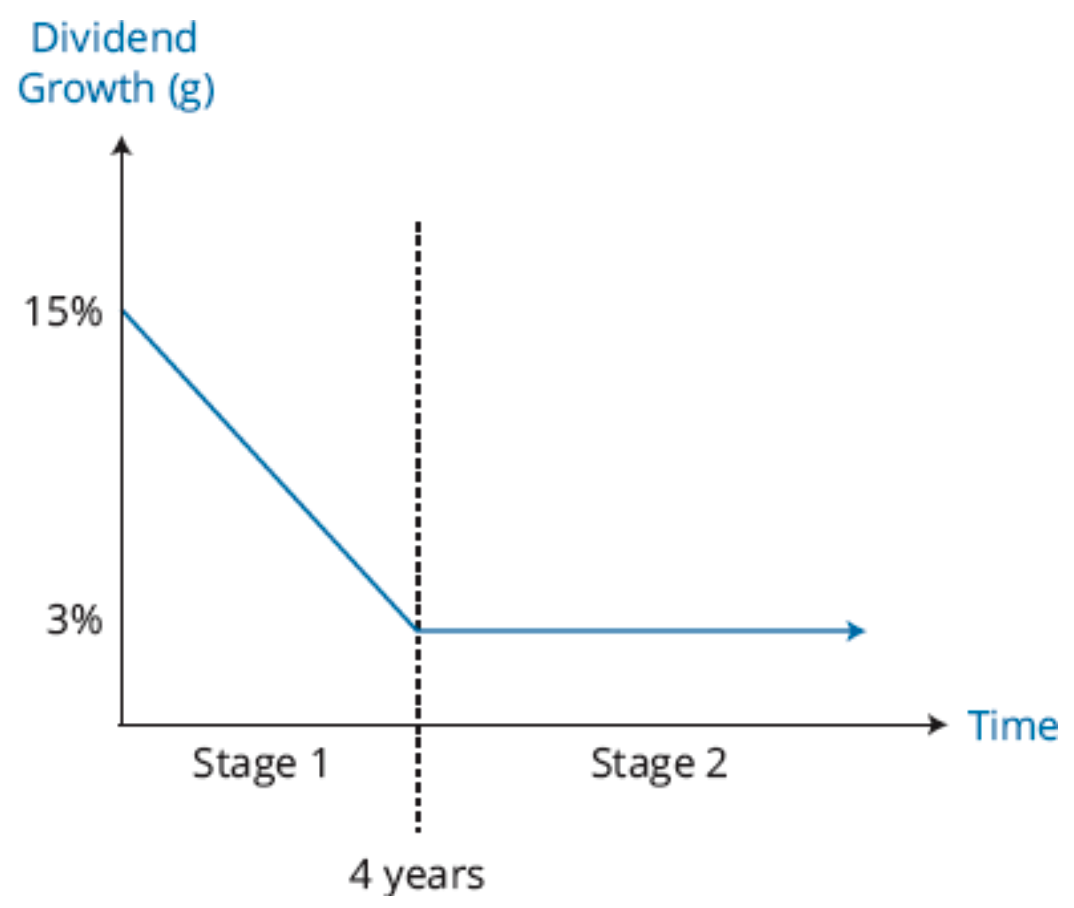
\includegraphics[scale=0.4]{images/equity/hmodel}
\caption{Example of a H-model}
\end{figure}

\begin{method} \hlt{Three-Stage Model DDM}\\
Firms that are expected to have three distinct stages of earnings growth.\\
More complex refinement of two-stage model. Process of using the model is as follows:
\begin{enumerate}[label=\roman*.]
\setlength{\itemsep}{0pt}
\item Gather the required inputs:
\begin{enumerate}[label=\arabic*.]
\setlength{\itemsep}{0pt}
\item the current dividend
\item estimate lengths of first, second, third stages and the expected growth rate in each stage
\item estimate of required return on equity
\end{enumerate}
\item compute the expected dividends in first stage and find sum of their present values. To investigate the company more deeply, such as explicit, individual earnings and dividend forecasts for the near future
\item apply H-model expression to second and third stages to obtain estimate of their value as beginning of second stage, then discount this H-value to as of $t=0$
\item sum the values obtained in the second and third steps
\end{enumerate}
\end{method}

\begin{figure}[H]
\centering
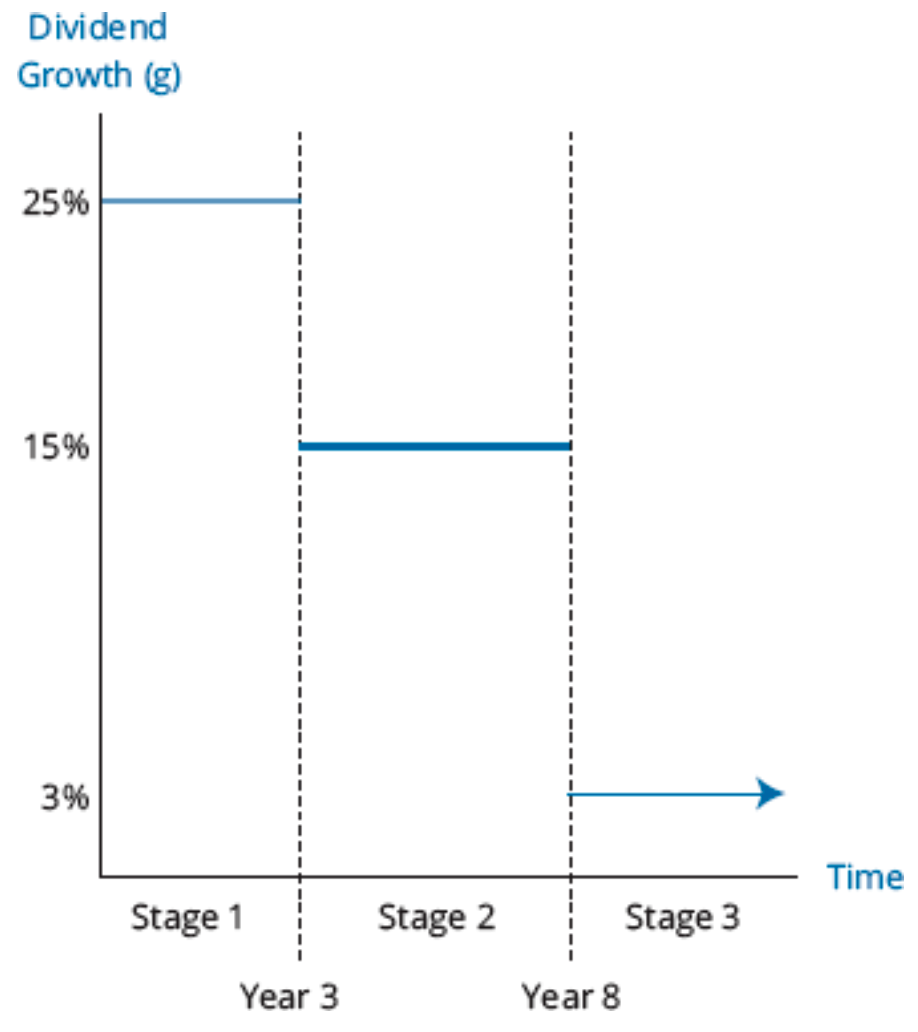
\includegraphics[scale=0.4]{images/equity/threestage}
\caption{Example of a three-stage model}
\end{figure}

\begin{method} \hlt{Terminal Value Estimation}
\begin{enumerate}[label=\roman*.]
\setlength{\itemsep}{0pt}
\item Gordon Growth Model: at some point in the future, assume dividends will grow at constant, long-term rate. The terminal value is then the value from Gordon Growth Model.
\item Market Price Multiples: forecast earnings and P/E ratio at the forecast horizon, then estimate the terminal value as the P/E multiplied by the earnings estimate.
\end{enumerate}
\end{method}

\begin{method} \hlt{Sustainable Growth Rate (SGR)}\\
Rate at which earnings (and dividends) can growth indefinitely, assuming debt-to-equity ratio is unchanged, and no new equity is issued.
\begin{equation}
SGD = b \times ROE \nonumber
\end{equation}
where $b$ is earnings return rate, equal to $1 - $ dividend payout rate.
\begin{enumerate}[label=\roman*.]
\setlength{\itemsep}{0pt}
\item Mature phase ROE may be estimated via:
\begin{enumerate}[label=\arabic*.]
\setlength{\itemsep}{0pt}
\item DuPont decomposition of ROE based on forecasts for components of DuPoint expression
\begin{align}
\text{ROE} &= \frac{\text{NI} - \text{Dividends}}{\text{NI}} \times \frac{\text{NI}}{\text{Sales}} \times \frac{\text{Sales}}{\text{Average assets}} \times \frac{\text{Average assets}}{\text{Average equity}} \nonumber
\end{align}
This is the \hlt{PRAT Model}, where SGR is function of profit margin (P), retention rate (R), asset turnover (A), financial leverage (T). Variables P and A are functions of performance, variables R and T are functions of financing decisions.\\
If actual growth rate is forecasted to be greater than SGR, the firm will have to issue equity unless the firm increases one of PRAT model factors.\\
For equity valuation, beginning-of-year BS values for mixed ratios are used.
\item Setting ROE $=r$, the require rate of return based on equity, on assumption that mature phase companies can do no more than earn investor's opportunity cost of capital
\item Setting ROE in mature phase equal to median industry ROE
\end{enumerate}
\item Relating $g$ to macroeconomic variables such as industry, growth, projections.
\end{enumerate}
\end{method}

\begin{definition} \hlt{Valuation of Stock}\\
If stock price is higher than model price, stock is overvalued.\\
If stock price is lower than model price, stock is undervalued.\\
If stock price is equal to model price, stock is fairly valued.
\end{definition}